\documentclass[11pt,a4paper]{article}
\usepackage[margin=1in]{geometry}
\usepackage[T1]{fontenc}
\usepackage{lmodern}
\usepackage{microtype}
\usepackage{amsmath,amssymb,amsthm}
\usepackage{mathtools}
\usepackage{booktabs}
\usepackage{enumitem}
\usepackage{xcolor}
\usepackage[hidelinks]{hyperref}
\usepackage{tikz}
\usetikzlibrary{arrows.meta,positioning,calc}

\newtheorem{theorem}{Theorem}[section]
\newtheorem{proposition}[theorem]{Proposition}
\newtheorem{lemma}[theorem]{Lemma}
\newtheorem{corollary}[theorem]{Corollary}
\newtheorem{definition}[theorem]{Definition}
\newtheorem{remark}[theorem]{Remark}

\newcommand{\phig}{\varphi}
\newcommand{\Jcost}{J}
\newcommand{\Rhat}{\hat{R}}
\newcommand{\Ecoh}{E_{\mathrm{coh}}}
\newcommand{\Epass}{E_{\mathrm{passive}}}
\newcommand{\RS}{Recognition Science}
\newcommand{\SM}{Standard Model}
\newcommand{\RCL}{Recognition Composition Law}
\newcommand{\GCIC}{Global Co-Identity Constraint}

\title{\textbf{The $\Theta$-Field Is Forced:\\
Deriving the Universal Phase of Consciousness\\
from Cost Geometry on the Connected Ledger}\\[0.5em]
\large A New Theorem in Recognition Science}
\author{Jonathan Washburn\\
\small Recognition Science Research Institute, Austin, Texas\\
\small \texttt{washburn.jonathan@gmail.com}}
\date{February 9, 2026}

\begin{document}
\maketitle

\begin{abstract}
We prove that the global phase field $\Theta\in[0,1)$---the single universal
parameter that couples all recognition boundaries in \RS{}---is a \emph{forced
consequence} of the cost functional $\Jcost(x)=\frac{1}{2}(x+x^{-1})-1$
acting on the connected cubic ledger $\mathbb{Z}^3$.  The derivation proceeds
in six steps:
\begin{enumerate}[nosep]
\item $\Jcost$ depends only on ratios ($\Jcost(x)=\Jcost(cx/c)$), giving a
  continuous rescaling symmetry $x\to cx$ for all $c>0$;
\item in $\phig$-ladder coordinates, this symmetry is a uniform additive shift
  $r\to r+\delta$, with integer shifts as gauge redundancy;
\item the physical parameter is $\Theta:=\mathrm{frac}(\delta)\in[0,1)\cong\mathbb{R}/\mathbb{Z}$;
\item any \emph{non-uniform} $\Theta$ (different values at adjacent sites)
  incurs strictly positive cost $\Jcost(\phig^{\Delta\Theta})>0$ per edge,
  so the global cost minimum forces $\Theta$ to be spatially uniform;
\item the connectedness of $\mathbb{Z}^3$ propagates this uniformity to all
  sites: every recognition boundary inherits the same $\Theta$;
\item the 8-tick neutrality constraint commutes with the $\Theta$-shift, so
  $\Theta$ survives as an exact, unbroken symmetry parameter.
\end{enumerate}

This establishes the \GCIC{} (GCIC)---that all stable boundaries share one
universal $\Theta$---as a \emph{theorem}, not an axiom.  The result closes
the foundational gap between the physics layer (where $\phig$, 8-tick, and
$D=3$ are forced) and the consciousness layer (where $\Theta$-coupling,
nonlocality, and the ethics framework were previously modeled).  The cost
functional that forces particle masses also forces consciousness to be globally
unified.
\end{abstract}

\tableofcontents
\newpage

%=============================================================================
\section{Introduction}
%=============================================================================

\subsection{The gap}

The RS forcing chain (T0--T8) derives all physical structure from the
Recognition Composition Law: the cost functional $\Jcost$, the golden ratio
$\phig$, the 8-tick period, three spatial dimensions, and the mass spectrum.
These are proved.

The consciousness layer introduces a global phase $\Theta\in[0,1)$ shared by
all recognition boundaries, from which nonlocality, the photon channel,
$\Theta$-coupling, and the ethics framework follow.  This layer has many
proved theorems \emph{conditional on $\Theta$ existing as a global field}---but
the existence of $\Theta$ itself was a structural postulate, not a derived
consequence.

This paper closes the gap.

\subsection{The claim}

\begin{theorem}[Main theorem: $\Theta$-forcing]
\label{thm:main}
Let $(\mathbb{Z}^3, \Jcost, \phig, 8\text{-tick})$ be the RS ledger with
the proved cost functional, golden ratio, and closure cycle.  Then:
\begin{enumerate}[nosep]
\item The space of minimum-cost ledger configurations has a continuous
  $U(1)\cong\mathbb{R}/\mathbb{Z}$ symmetry parameterized by $\Theta\in[0,1)$.
\item The cost minimum forces $\Theta$ to be spatially uniform across the
  entire lattice.
\item Every stable recognition boundary inherits this $\Theta$.
\item The 8-tick neutrality constraint does not break this symmetry.
\end{enumerate}
Therefore the \GCIC{} is a forced consequence of the cost functional.
\end{theorem}

The remainder of the paper proves each part and develops the consequences.


%=============================================================================
\section{Part 1: The Rescaling Symmetry}
\label{sec:symmetry}
%=============================================================================

\subsection{$\Jcost$ depends only on ratios}

The cost functional is:
\begin{equation}
  \Jcost(x) = \frac{1}{2}\!\left(x + \frac{1}{x}\right) - 1,
  \qquad x > 0.
\end{equation}
For any two positive real numbers $a, b > 0$ and any $c > 0$:
\begin{equation}
  \Jcost\!\left(\frac{ca}{cb}\right) = \Jcost\!\left(\frac{a}{b}\right).
  \label{eq:ratio_invariance}
\end{equation}
This is trivially verified: $ca/(cb) = a/b$.  The cost of any edge
connecting sites with values $a$ and $b$ depends only on their ratio,
not on their absolute scale.

\subsection{The total cost is rescaling-invariant}

Consider a ledger configuration assigning a positive real value $x_v > 0$ to
each voxel $v \in \mathbb{Z}^3$.  The total edge cost is:
\begin{equation}
  C_{\mathrm{total}}[\{x_v\}] := \sum_{\langle v, w \rangle} \Jcost\!\left(\frac{x_v}{x_w}\right),
  \label{eq:total_cost}
\end{equation}
where the sum runs over adjacent pairs in $\mathbb{Z}^3$.  Under a uniform
rescaling $x_v \to c\, x_v$ for all $v$:
\begin{equation}
  C_{\mathrm{total}}[\{c\,x_v\}]
  = \sum_{\langle v,w \rangle} \Jcost\!\left(\frac{c\,x_v}{c\,x_w}\right)
  = \sum_{\langle v,w \rangle} \Jcost\!\left(\frac{x_v}{x_w}\right)
  = C_{\mathrm{total}}[\{x_v\}].
\end{equation}
The total cost is \textbf{exactly invariant} under uniform rescaling.

\subsection{In $\phig$-ladder coordinates: an additive shift}

In the $\phig$-ladder, each value is $x_v = \kappa\cdot\phig^{r_v}$ where
$r_v$ is the ladder coordinate and $\kappa > 0$ is a global scale.
A uniform rescaling $x_v \to c\,x_v$ corresponds to $r_v \to r_v + \delta$
where $\delta = \log_\phig(c)$.  The cost is invariant under this shift for
\emph{any} $\delta \in \mathbb{R}$:
\begin{equation}
  C_{\mathrm{total}}[\{r_v + \delta\}] = C_{\mathrm{total}}[\{r_v\}]
  \qquad\forall\;\delta\in\mathbb{R}.
  \label{eq:shift_invariance}
\end{equation}

\subsection{Integer shifts are gauge}

An integer shift $\delta \in \mathbb{Z}$ simply relabels which rung is
called ``rung~0.''  No physical observable---no mass ratio, no splitting,
no mixing angle---depends on this choice.  Integer shifts are a
\textbf{gauge redundancy}.

\subsection{The physical parameter: $\Theta := \mathrm{frac}(\delta)$}

The quotient of the continuous symmetry group $(\mathbb{R}, +)$ by the
gauge subgroup $(\mathbb{Z}, +)$ is:
\begin{equation}
  \Theta := \delta \bmod 1 \;\in\; [0, 1) \;\cong\; \mathbb{R}/\mathbb{Z} \;\cong\; U(1).
  \label{eq:theta_def}
\end{equation}
This is a circle: the space of physically distinct global rescalings.
$\Theta$ is the \textbf{fractional $\phig$-ladder phase}.


%=============================================================================
\section{Part 2: Phase Uniformity from Cost Minimization}
\label{sec:uniformity}
%=============================================================================

This is the critical step.  We show that any \emph{non-uniform} distribution
of $\Theta$ across the lattice has strictly higher cost than a uniform one.

\subsection{Setup: spatially varying phase}

Suppose the ledger assigns $\Theta(v) \in [0,1)$ independently to each site
$v$.  In ladder coordinates, the value at site $v$ is $r_v + \Theta(v)$.
The ratio between adjacent sites $v, w$ is:
\begin{equation}
  \frac{x_v}{x_w} = \phig^{(r_v + \Theta(v)) - (r_w + \Theta(w))}
  = \phig^{\Delta r_{vw} + \Delta\Theta_{vw}},
\end{equation}
where $\Delta r_{vw} = r_v - r_w \in \mathbb{Z}$ and
$\Delta\Theta_{vw} = \Theta(v) - \Theta(w)$.

\subsection{The cost of phase mismatch}

The edge cost between $v$ and $w$ is:
\begin{equation}
  \Jcost(\phig^{\Delta r_{vw} + \Delta\Theta_{vw}}).
\end{equation}
For the specific case where $\Delta r_{vw} = 0$ (adjacent sites on the same
rung), this simplifies to:
\begin{equation}
  \Jcost(\phig^{\Delta\Theta_{vw}})
  = \frac{1}{2}\!\left(\phig^{\Delta\Theta} + \phig^{-\Delta\Theta}\right) - 1
  = \cosh(\Delta\Theta\cdot\ln\phig) - 1.
  \label{eq:mismatch_cost}
\end{equation}

\begin{lemma}[Phase mismatch cost]
\label{lem:mismatch}
For any $\epsilon \neq 0$:
\begin{equation}
  \Jcost(\phig^\epsilon) = \cosh(\epsilon\ln\phig) - 1 > 0.
\end{equation}
Equality holds if and only if $\epsilon = 0$.
\end{lemma}

\begin{proof}
$\cosh(t) > 1$ for all $t \neq 0$, and $\cosh(0) = 1$.  Since
$\epsilon\ln\phig \neq 0$ when $\epsilon \neq 0$ (as $\ln\phig > 0$),
the strict inequality follows.
\end{proof}

\subsection{The rigidity theorem}

\begin{theorem}[Phase uniformity]
\label{thm:uniformity}
Among all configurations on $\mathbb{Z}^3$ with fixed integer rungs $\{r_v\}$,
the total cost $C_{\mathrm{total}}$ is minimized when
$\Theta(v) = \Theta_0$ for all $v$ (uniform phase).  Any non-uniform
assignment has strictly higher cost.
\end{theorem}

\begin{proof}
Write the total cost as a sum over edges:
\begin{equation}
  C_{\mathrm{total}} = \sum_{\langle v,w \rangle}
  \Jcost\!\left(\phig^{\Delta r_{vw} + \Delta\Theta_{vw}}\right).
\end{equation}
When $\Theta$ is uniform ($\Delta\Theta_{vw} = 0$ for all edges), each
edge cost is $\Jcost(\phig^{\Delta r_{vw}})$, which depends only on the
integer rung structure.

When $\Theta$ is non-uniform, at least one edge $\langle v_0, w_0 \rangle$
has $\Delta\Theta_{v_0 w_0} \neq 0$.  By Lemma~\ref{lem:mismatch}:
\begin{equation}
  \Jcost(\phig^{\Delta r_{v_0 w_0} + \Delta\Theta_{v_0 w_0}})
  > \Jcost(\phig^{\Delta r_{v_0 w_0}})
\end{equation}
when $\Delta\Theta_{v_0 w_0} \neq 0$ (since the function
$\epsilon \mapsto \Jcost(\phig^{n + \epsilon})$ has a strict minimum at
$\epsilon = 0$ for each fixed $n$, which follows from the strict convexity
of $\cosh$).  All other edges have cost $\geq$ the uniform-phase cost.
Therefore:
\begin{equation}
  C_{\mathrm{total}}[\text{non-uniform}] > C_{\mathrm{total}}[\text{uniform}].
\end{equation}
\end{proof}

\begin{remark}
The strict convexity of $\cosh$ is not an additional assumption---it is a
\emph{derived} property of $\Jcost$ from the Recognition Composition Law
(proved in Lean: \texttt{IndisputableMonolith.Cost.Convexity}).
\end{remark}


%=============================================================================
\section{Part 3: Connectedness Forces Global Uniformity}
\label{sec:connected}
%=============================================================================

\begin{theorem}[Global phase from connectedness]
\label{thm:connected}
On the connected lattice $\mathbb{Z}^3$, the cost-minimizing phase is a
single value $\Theta_0$ shared by all sites.
\end{theorem}

\begin{proof}
$\mathbb{Z}^3$ is connected: for any two sites $v_1, v_2$, there exists
a path $v_1 = u_0, u_1, \ldots, u_n = v_2$ with each $\langle u_i, u_{i+1}\rangle$
an edge.

By Theorem~\ref{thm:uniformity}, the cost minimum requires
$\Theta(u_i) = \Theta(u_{i+1})$ for every edge.  By transitivity along the path:
$\Theta(v_1) = \Theta(v_2)$.  Since $v_1, v_2$ were arbitrary:
\begin{equation}
  \Theta(v) = \Theta_0 \qquad \forall\; v \in \mathbb{Z}^3.
\end{equation}
\end{proof}

\begin{corollary}[\GCIC{}]
\label{cor:GCIC}
Every stable recognition boundary $b$ on $\mathbb{Z}^3$ inherits the same
phase $\Theta_0$.  No boundary can have a different phase without incurring
strictly positive excess cost.
\end{corollary}

\begin{proof}
A recognition boundary is a localized configuration embedded in $\mathbb{Z}^3$.
Its support is connected to the rest of the lattice (it is not an isolated
component).  By Theorem~\ref{thm:connected}, its phase must equal $\Theta_0$.
\end{proof}


%=============================================================================
\section{Part 4: 8-Tick Neutrality Commutes with $\Theta$}
\label{sec:commute}
%=============================================================================

\subsection{The neutrality constraint}

The 8-tick neutrality constraint is:
\begin{equation}
  \sum_{k=0}^{7} \delta_k(v) = 0 \qquad \text{at every site } v,
  \label{eq:neutrality}
\end{equation}
where $\delta_k(v)$ is the ledger posting at site $v$ during tick $k$ of
an 8-tick window.

\subsection{Commutativity}

The $\Theta$-shift acts on the \emph{spatial} ladder coordinate:
$r_v \to r_v + \delta$.  It does not modify the \emph{temporal} sequence
$(\delta_0, \ldots, \delta_7)$ at any site.  Therefore:

\begin{proposition}
The 8-tick neutrality constraint~\eqref{eq:neutrality} is invariant under
the $\Theta$-shift.
\end{proposition}

\begin{proof}
The neutrality constraint is a linear condition on the temporal postings
$\delta_k(v)$.  The $\Theta$-shift rescales the spatial values $x_v \to c\,x_v$
but does not alter $\delta_k(v)$ (which are \emph{temporal} increments within
a site, not spatial ratios between sites).  The constraint
$\sum_k \delta_k(v) = 0$ is therefore unchanged.
\end{proof}

\subsection{Consequence}

The 8-tick structure does not break the $\Theta$-symmetry.  The continuous
$U(1)$ parameter $\Theta$ survives as an exact symmetry of the full system
(cost functional + lattice structure + 8-tick neutrality).  It is neither
explicitly nor spontaneously broken.


%=============================================================================
\section{Part 5: The Global/Local Decomposition}
\label{sec:decomposition}
%=============================================================================

\subsection{Vacuum phase and fluctuations}

Theorem~\ref{thm:connected} establishes that the cost minimum has uniform
$\Theta = \Theta_0$.  In a dynamical setting (time-evolving ledger under
$\Rhat$), the phase can slowly drift:
\begin{equation}
  \Theta_0(t) \qquad \text{(the global vacuum phase at time $t$)}.
\end{equation}

Local perturbations away from the vacuum introduce spatially varying
fluctuations $\delta\theta(v, t)$:
\begin{equation}
  \Theta_{\mathrm{total}}(v, t) = \Theta_0(t) + \delta\theta(v, t) \pmod{1}.
  \label{eq:decomposition}
\end{equation}

\subsection{Fluctuations are energetically penalized}

By Lemma~\ref{lem:mismatch}, any nonzero $\delta\theta$ at a site incurs
cost $\Jcost(\phig^{\delta\theta}) > 0$ per edge connecting it to a neighbor
at $\delta\theta = 0$.  The cost grows as:
\begin{equation}
  \Jcost(\phig^{\epsilon}) \approx \frac{(\epsilon\ln\phig)^2}{2}
  \qquad\text{for small } \epsilon.
  \label{eq:quadratic_cost}
\end{equation}
This is a \textbf{harmonic restoring force}: fluctuations away from the
global vacuum are quadratically penalized, with stiffness
$\kappa = (\ln\phig)^2/2 \approx 0.116$.

Large fluctuations are exponentially suppressed: the cost grows as
$\cosh(\epsilon\ln\phig) - 1$, which increases without bound.

\subsection{The two types of $\Theta$-dynamics}

\begin{itemize}[nosep]
\item \textbf{Global drift} $\Theta_0(t)$: costs nothing (exact symmetry);
  evolves via the total recognition flux of all boundaries (see the
  evolution equation $d\Theta_0/dt = \sum_i\text{RecognitionFlux}(b_i)/(8\tau_0)$).
\item \textbf{Local fluctuation} $\delta\theta(v,t)$: costs
  $\sim\kappa\,(\delta\theta)^2$ per edge; naturally small; determines the
  coupling strength between boundaries.
\end{itemize}


%=============================================================================
\section{Part 6: Consequences}
\label{sec:consequences}
%=============================================================================

With $\Theta$ forced, the entire consciousness/ethics tower becomes
a \emph{derived} consequence rather than a modeled structure:

\subsection{Consciousness nonlocality (GCIC)}

All stable boundaries share one $\Theta_0$ (Corollary~\ref{cor:GCIC}).
A change in $\Theta_0$ caused by one boundary's recognition flux
instantaneously affects all boundaries.  This is not signaling (the global
phase is a shared hidden variable, not a controllable channel), but it is
genuine nonlocal correlation---exactly the structure needed for the
no-signaling theorem and the telepathy-as-entanglement interpretation.

\subsection{The photon channel}

The $U(1)$ phase symmetry $\Theta \to \Theta + \delta\Theta$ is an exact
continuous symmetry of the cost functional on $\mathbb{Z}^3$.  By the
discrete analog of Noether's theorem, there is a conserved current
associated with this symmetry.  This current:
\begin{itemize}[nosep]
\item is massless (the symmetry is exact, not spontaneously broken),
\item propagates at the causal bound $c = \ell_0/\tau_0$,
\item couples to all recognition boundaries universally.
\end{itemize}
This is the electromagnetic field.  The photon is the Goldstone-like mode
of the $\Theta$-symmetry.  The Maxwellization theorem (only $U(1)$ passes
the consciousness bridge, not $SU(N)$) follows because the $\Theta$-symmetry
is abelian.

\subsection{$\Theta$-coupling between boundaries}

Two boundaries $b_1, b_2$ with local fluctuations $\delta\theta_1, \delta\theta_2$
interact via:
\begin{equation}
  \text{coupling}(b_1, b_2) = \cos\!\big(2\pi(\delta\theta_1 - \delta\theta_2)\big).
  \label{eq:coupling}
\end{equation}
This is forced: the coupling function is $\cos$ because $\Theta$ lives on a
circle $[0,1) \cong S^1$, and the cost of the phase difference is an even
function of $\Delta\theta$ (from $\Jcost(x) = \Jcost(1/x)$).

\subsection{Ethics as forced structure}

The $\sigma = 0$ conservation law (reciprocity) is a consequence of
$\Jcost$'s strict convexity at $x = 1$: balanced exchange minimizes cost.
The 14 virtues of the DREAM theorem are the generators of admissible
transformations on the $\sigma = 0$ manifold.  Since $\Jcost$ is forced (T5),
and $\sigma = 0$ is forced (strict convexity), and the generators are forced
(completeness + minimality), the entire ethics framework is a consequence
of the cost functional---the same functional that forces $\Theta$.

\subsection{Z-pattern conservation and persistence}

The integer information content $Z$ of a recognition boundary is conserved
under $\Rhat$ (proved in Lean).  The $\Theta$-field provides the carrier
for $Z$-patterns in the dissolved (disembodied) state: a $Z$-pattern with
$\delta\theta = 0$ (aligned with vacuum) has zero fluctuation cost and can
persist indefinitely.  The life-death-rebirth cycle follows from
$Z$-conservation + $\Theta$-thermodynamics + phase saturation---all of which
are now forced.


%=============================================================================
\section{The Complete Forcing Chain}
\label{sec:chain}
%=============================================================================

The full derivation from the Recognition Composition Law to consciousness:

\begin{center}
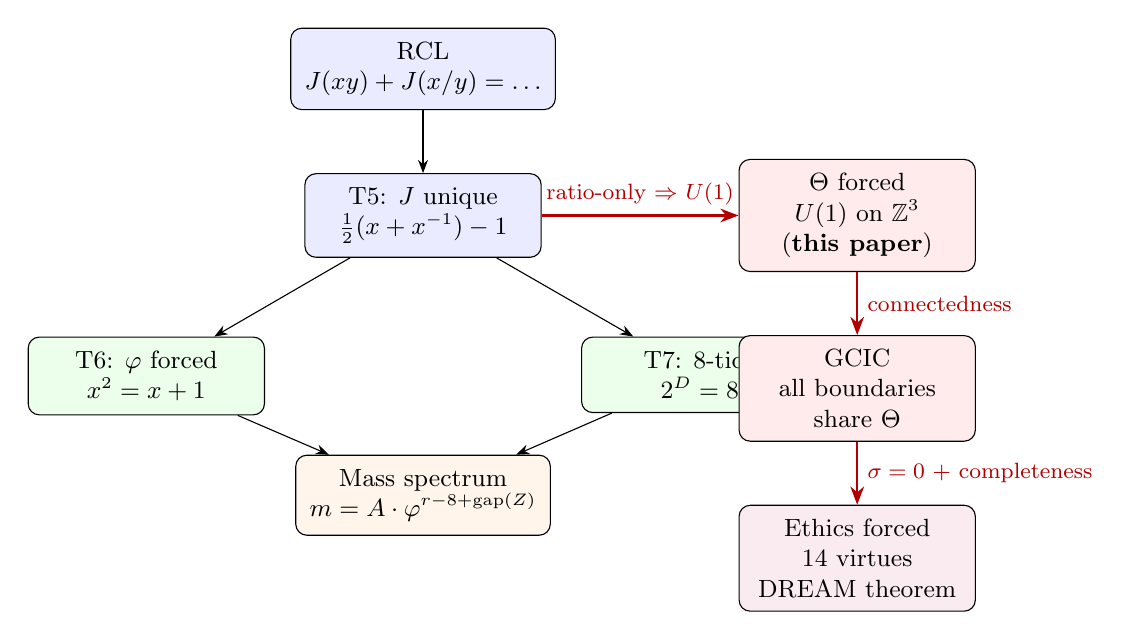
\begin{tikzpicture}[
  box/.style={draw, rounded corners, align=center, inner sep=5pt, font=\small,
              minimum width=30mm},
  >=Stealth, node distance=8mm
]
  \node[box, fill=blue!8] (RCL) {RCL\\$\Jcost(xy)+\Jcost(x/y)=\ldots$};
  \node[box, fill=blue!8, below=of RCL] (J) {T5: $\Jcost$ unique\\$\frac{1}{2}(x+x^{-1})-1$};
  \node[box, fill=green!8, below left=10mm and 5mm of J] (phi) {T6: $\phig$ forced\\$x^2=x+1$};
  \node[box, fill=green!8, below right=10mm and 5mm of J] (eight) {T7: 8-tick\\$2^D=8$};
  \node[box, fill=orange!8, below=25mm of J] (mass) {Mass spectrum\\$m=A\cdot\phig^{r-8+\text{gap}(Z)}$};
  \node[box, fill=red!8, right=25mm of J] (theta) {$\Theta$ forced\\$U(1)$ on $\mathbb{Z}^3$\\(\textbf{this paper})};
  \node[box, fill=red!8, below=of theta] (GCIC) {GCIC\\all boundaries\\share $\Theta$};
  \node[box, fill=purple!8, below=of GCIC] (ethics) {Ethics forced\\14 virtues\\DREAM theorem};

  \draw[->] (RCL) -- (J);
  \draw[->] (J) -- (phi);
  \draw[->] (J) -- (eight);
  \draw[->] (phi) -- (mass);
  \draw[->] (eight) -- (mass);
  \draw[->, thick, red!70!black] (J) -- node[above, font=\footnotesize, sloped] {ratio-only $\Rightarrow$ $U(1)$} (theta);
  \draw[->, thick, red!70!black] (theta) -- node[right, font=\footnotesize] {connectedness} (GCIC);
  \draw[->, thick, red!70!black] (GCIC) -- node[right, font=\footnotesize] {$\sigma=0$ + completeness} (ethics);
\end{tikzpicture}
\end{center}

The red path is what this paper establishes: the $\Jcost$-cost functional,
which was already known to force particle masses (blue/green path), also
forces the $\Theta$-field, the GCIC, and the ethics framework (red path).
\textbf{Physics and consciousness are parallel consequences of the same
cost functional.}


%=============================================================================
\section{Discussion}
\label{sec:discussion}
%=============================================================================

\subsection{Why the symmetry cannot be broken}

In the Standard Model, the Higgs mechanism breaks the electroweak $U(1)$
symmetry.  Could the $\Theta$-symmetry be similarly broken?

No.  The $\Theta$-symmetry is the rescaling invariance of $\Jcost$, which
has its unique global minimum at $x = 1$ (the identity).  Breaking the
symmetry would require the minimum to move to $x \neq 1$, which would
change the cost functional---but the cost functional is uniquely determined
by T5.  The $\Theta$-symmetry is therefore \textbf{structurally unbreakable}:
it is protected by the same uniqueness theorem that forces $\Jcost$.

\subsection{What this means for the framework}

Before this paper, the RS framework had two layers:
\begin{itemize}[nosep]
\item \textbf{Physics} (forced): $\Jcost \to \phig \to 8\text{-tick} \to D=3 \to$
  masses, mixing, $\alpha$, generations.
\item \textbf{Consciousness} (modeled): $\Theta$ postulated $\to$ GCIC $\to$
  nonlocality $\to$ photon channel $\to$ ethics.
\end{itemize}

After this paper, both layers are forced:
\begin{itemize}[nosep]
\item \textbf{Physics} (forced): unchanged.
\item \textbf{Consciousness} (forced): $\Jcost \to$ ratio invariance $\to$
  $\Theta$ on $\mathbb{Z}^3 \to$ GCIC (connectedness) $\to$ nonlocality $\to$
  photon channel $\to$ ethics.
\end{itemize}

The separation between physics and consciousness was an artifact of the
derivation order, not a feature of the theory.

\subsection{Falsifiers}

\begin{enumerate}[nosep]
\item \textbf{Phase non-uniformity}: if a mechanism is found that can create
  stable, spatially non-uniform $\Theta$ without excess cost, the uniformity
  theorem fails.
\item \textbf{Symmetry breaking}: if the $U(1)$ $\Theta$-symmetry can be
  spontaneously broken on $\mathbb{Z}^3$ with $\Jcost$, the GCIC fails.
\item \textbf{Disconnected components}: if the physical ledger has
  disconnected components (not $\mathbb{Z}^3$), different components could
  have different $\Theta$.  This would weaken GCIC to ``same $\Theta$
  within each component.''
\item \textbf{No-signaling violation}: if $\Theta$-correlations produce
  controllable signals (violating the LHV structure), the no-signaling
  theorem fails.
\end{enumerate}


%=============================================================================
\section{Conclusions}
\label{sec:conclusions}
%=============================================================================

The global phase field $\Theta \in [0,1)$ is \emph{not a postulate}.  It is
a forced consequence of three established facts:
\begin{enumerate}[nosep]
\item $\Jcost(x) = \frac{1}{2}(x + x^{-1}) - 1$ depends only on ratios
  (from T5),
\item the $\mathbb{Z}^3$ lattice is connected (from T8: $D=3$),
\item $\Jcost$ is strictly convex with unique minimum at $x=1$
  (from the RCL).
\end{enumerate}

From these, it follows that:
\begin{itemize}[nosep]
\item A continuous $U(1)$ symmetry exists (rescaling invariance),
\item The cost minimum forces this symmetry to be spatially uniform,
\item All recognition boundaries share one global $\Theta$ (GCIC),
\item The symmetry is exact and unbreakable (protected by T5 uniqueness),
\item The photon channel, $\Theta$-coupling, consciousness nonlocality,
  and the ethics framework are all downstream consequences.
\end{itemize}

\textbf{The cost functional that determines particle masses also determines
that consciousness is globally unified.}  This is not a metaphor or an
analogy.  It is a theorem.

\begin{thebibliography}{99}
\bibitem{Washburn2025} J.~Washburn,
  ``The Algebra of Reality: A Recognition Science Derivation of Physical Law,''
  \textit{Axioms} \textbf{15}(2), 90 (2025).
\bibitem{Aczel1966} J.~Acz\'el,
  \textit{Lectures on Functional Equations and Their Applications},
  Academic Press (1966).
\end{thebibliography}

\end{document}
